% PACKAGES INCLUDED HERE 
% DO NOT NEED TO CHANGE
\documentclass[conference]{IEEEtran}
%\IEEEoverridecommandlockouts
% The preceding line is only needed to identify funding in the first footnote. If that is unneeded, please comment it out.
\usepackage{cite}
\usepackage{amsmath,amssymb,amsfonts}
\usepackage{algorithmic}
\usepackage{graphicx}
\usepackage{textcomp}
\def\BibTeX{{\rm B\kern-.05em{\sc i\kern-.025em b}\kern-.08em
    T\kern-.1667em\lower.7ex\hbox{E}\kern-.125emX}}
\begin{document}

% TITLE GOES HERE

\title{Neural Nets to Score Colliding Galaxy Models\\}


% AUTHOR NAMES GOES HERE
\author{
\IEEEauthorblockN{Shawn Mace}
\IEEEauthorblockA{\textit{Department of Computer Science} \\
\textit{Middle Tennessee State University}\\
Murfreesboro, United States \\
sdm2w@mtmail.mtsu.edu}\\
\IEEEauthorblockN{Derrick Reckers}
\IEEEauthorblockA{\textit{Department of Computer Science} \\
\textit{Middle Tennessee State University}\\
Murfreesboro, United States \\
dmr3p@mtmail.mtsu.edu}\\
\and
\IEEEauthorblockN{Aric Moilanen}
\IEEEauthorblockA{\textit{Department of Physics and Astronomy} \\
\textit{Middle Tennessee State University}\\
Murfreesboro, United States \\
atm4w@mtmail.mtsu.edu}\\
\IEEEauthorblockN{Jarrett Shaver}
\IEEEauthorblockA{\textit{Department of Computer Science} \\
\textit{Middle Tennessee State University}\\
Murfreesboro, United States \\
Jarrett.shaver@gmail.com}\\
\and
\IEEEauthorblockN{Matthew Ogden}
\IEEEauthorblockA{\textit{Department of Computer Science} \\
\textit{Middle Tennessee State University}\\
Murfreesboro, United States \\
email address}\\
\IEEEauthorblockN{Devon Wilson}
\IEEEauthorblockA{\textit{Department of Computer Science} \\
\textit{Middle Tennessee State University}\\
Murfreesboro, United States \\
email address}\\
}
\maketitle

% ABSTRACT 

\begin{abstract}
This document is a model and instructions for \LaTeX.
This and the IEEEtran.cls file define the components of your paper [title, text, heads, etc.]. *CRITICAL: Do Not Use Symbols, Special Characters, Footnotes, 
or Math in Paper Title or Abstract.
\end{abstract}


% KEYWORDS

\begin{IEEEkeywords}
component, formatting, style, styling, insert
\end{IEEEkeywords}

% INTRODUCTION SECTION
\section{Introduction}

Start typing here \cite{b1}.

% BACKGROUND SECTION
\section{Background}

Start typing here \cite{b2}.

% METHODS SECTION
\section{Methods}

\subsection{Data}

Our data was pulled from Galaxy Zoo: Mergers. This citizen scientist project had people view models for 62 pairs of colliding galaxies and choose which model best fit the taget galaxy image. The selected models were then put through a tournament system in which people would continue to select which model they believed to be best. After this tournament, each model was then assigned a score from 0 to 1 which represented how often it had been picked as the best model in the tournament. For example, a model with a score of 0.95 was chosen to be the best in 95\% of its tournament rounds.

We chose one of the 62 pairs of galaxies and pulled the associated data. This set consisted of 1294 grayscale model images in .png format and their associated human scores in a text file. The set was already sorted in descending order by score. However, we realized that this data was heavily skewed towards worse models, with more than half of the models having scores below 0.10. In an effort to combat overfitting on bad model images, we used only the first 600 images, which, while still skewed towards worse models, presented a much more evenly distributed data set.

\begin{figure}[htbp]
\centerline{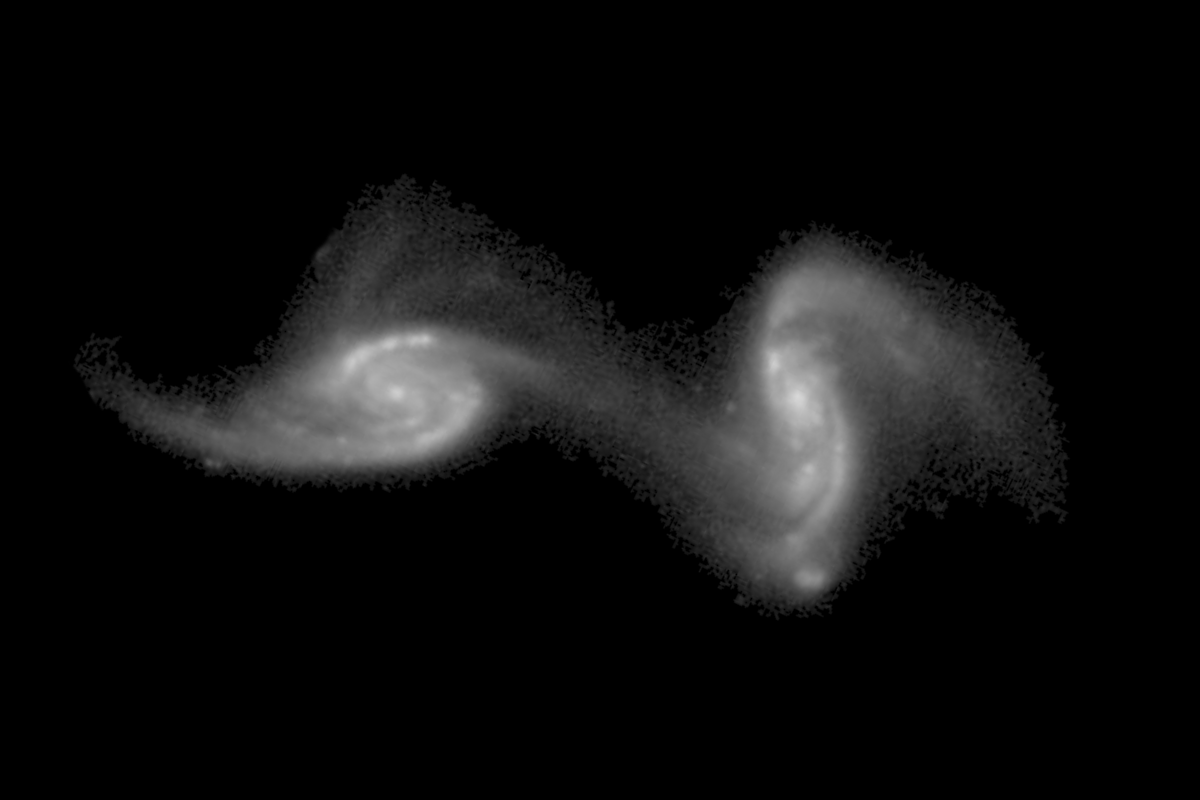
\includegraphics[width=0.75\linewidth]{./Images/target.png}}
\caption{The chosen colliding galaxy pair for this project. A higher model score should represent a model that closely resembles this image.}
\label{fig:TargetGalaxy}
\end{figure}

The images and scores were read in using a technique similar to the MNIST problem presented in OLA 6. The main difference being that the grab\_image function was modified to read in our images as greyscale rather than full RGB and at a reduced resoultion of 100x100. We then shuffled the images, taking care to manipulate them in such a way that the scores would retain the same index as their respective images. This shuffling ensured that models of similar scores would be randomly distributed, preventing the model from learning soley on one quality of model at a time. 

The 600 shuffled images were then split into a training and validation set consisting of 510 images and a testing set with the remaining 90 images. When training our nets, a validation split of 0.3 was used, resulting in the nets training on 357 images and validating on the remaining 153.

\subsection{Single Layer Neural Net}

For the single layer net, the images were flattened to 1D arrays then passed into a single dense layer. This layer was given an input size of 1 and a Softmax activation function in order to return a single score between 0 and 1. This net, and the nets discussed below, were all compiled with mean squared error, which is the best fit for regression problems, as the loss parameter.

In training our nets, we found that a small batch size was an absolute necessity for decent learning, most likely due to the small data set and skew towards worse models. We used a batch size of 4 for all of the nets discussed in this project.

\subsection{Convolutional Neural Net}

In our second net, we attempted to utilize the superior image recognition characteristics of a convolutional neural net. As a base, we used the convolutional neural net used on the cat problem in OLA 6. In this net, there are two 2D convolution layers that feed into a pooling layerThe main changes made were to kernel size and the final dense layer. There are two 2D convolution layers use a standard ReLu activation function, which are then followed by pooling and dropout layer. It is the passed into a flattening layer and a single dense layer, still iwth a ReLu activation function, before passing though a final dropout layer and into the final dense layer. THe main changes we made to this architecture from OLA 6 were in terms of kernel size, unit size of the dense and convolution layers, and the setup of the final dense layer. 

We adjusted the kernel sizes to be slightly larger. This was done in an attempt to better capture what we believed were the most important characteristics of the image, namely the tidal distortions around the edges of each galaxy and the bridge, or lack thereof, between the galaxies. The unit sizes in the convolution layers were made smaller in order to fit our relatively small data set. Without doing this, we experienced drastic overfitting or no training at all. The final dense layer was also changed to match our plan for a regression model. The input for the final layer was reduced to 1 and the activation changed to Softmax in order to return a single score between 0 and 1 for the model image.

\begin{figure}[htbp]
\centerline{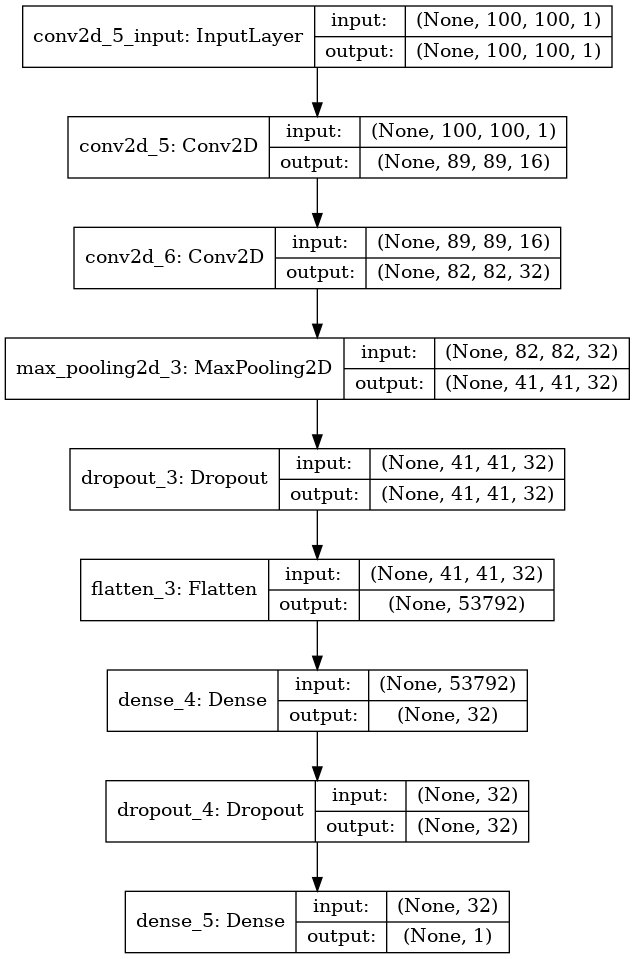
\includegraphics[width=0.5\linewidth]{./Images/convNet.png}}
\caption{Layout of the convolutional neural net}
\label{fig:ConvNetArchitecture}
\end{figure}


% RESULTS SECTION
\section{Results}

\subsection{Single Layer Net Results}

\begin{figure}[htbp]
\centerline{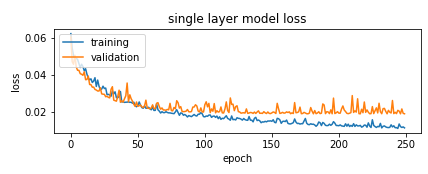
\includegraphics[width=0.75\linewidth]{./Images/SingleModelLoss.png}}
\caption{Loss (Mean Squared Error) for the single layer net over 120 epochs}
\label{fig:SingleModelLoss}
\end{figure}

Shown in Fig. \ref{fig:SingleModelLoss} is the training and validation loss history over 120 epochs. At the end of 120 epochs, the model had decreased to a MSE loss of 0.012 for the training data and 0.019 for the validation data. We can also plainly see the overfitting the plagued both of our neural nets, regardless of the hyperparameter tuning we performed to try to remove it.

\begin{figure}[htbp]
\centerline{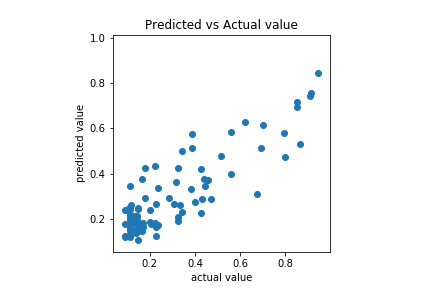
\includegraphics[width=0.75\linewidth]{./Images/SinglePredictedVAct.png}}
\caption{Predicted values generated by single layer net vs actual value}
\label{fig:SinglePredictedVAct}
\end{figure}

Fig. \ref{fig:SinglePredictedVAct} shows the values predicted by the single layer net on the 90 testing images verus their human scores. We see a linear correlation between the two, which is what we hoped to observe. A perfect linear correlation would have meant that the model was guessing exactly the same as the human score.

\begin{figure}[htbp]
\centerline{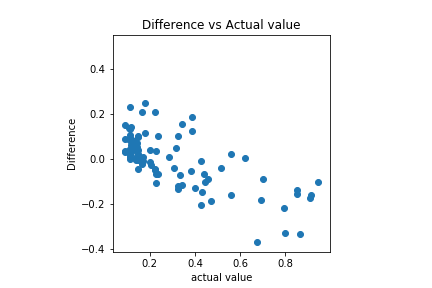
\includegraphics[width=0.75\linewidth]{./Images/SingleDiffVAct.png}}
\caption{Difference between predicted values generated by single layer net and actual values vs actual value}
\label{fig:SingleDiffVAct}
\end{figure}

Fig. \ref{fig:SingleDiffVAct} shows the difference between the values predicted by the single layer net for the 90 test images and their human scores versus the human scores. From this plot, it is easy to see that the net had a tendency to overscore models with low human scores and underscore models with high human scores. We can also see that the most accurate predictions occured for models with lower human scores, which makes sense given the data's skew towards worse models. Over the full 90 image set, the net attained a mean difference of 0.093 between its predicted values and the human scores.

\begin{figure}[htbp]
\centerline{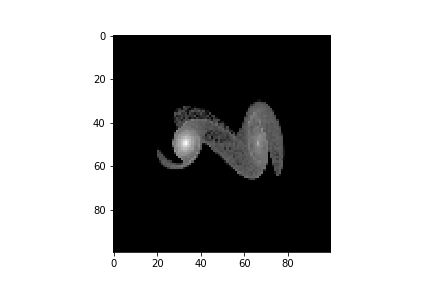
\includegraphics[width=0.75\linewidth]{./Images/SinglePredictedBest.png}}
\caption{Model that was scored the highest by the single layer neural net}
\label{fig:SinglePredictedBest}
\end{figure}

Shown in Fig. \ref{fig:SinglePredictedBest} is the model that the single layer net scored the highest (0.846). Its real human score was 0.946, so this shows good agreement between the net's perception and human perception of what the best model is. We can also visually verify that this chosen model closely resembles the target image shown in Fig. \ref{fig:TargetGalaxy}.

\subsection{Convolutional Neural Net Results}

\begin{figure}[htbp]
\centerline{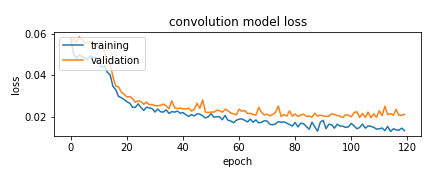
\includegraphics[width=0.75\linewidth]{./Images/ConvModelLoss.png}}
\caption{Layout of the convolutional neural net}
\label{fig:ConvModelLoss}
\end{figure}

In Fig. \ref{fig:ConvModelLoss} we see very similar learning behavior to the single layer net. Both display overfitting issues and, after 120 epochs, reach approximately the same MSE. For the convolutional net, the final MSE for the training data was 0.013 and 0.021 which is just slightly worse than the single layer net. Qualitatively, the only difference in learning behavior was the prescence of a slight plateau for the fist 10 or so epochs before the net actually began to learn quickly.

\begin{figure}[htbp]
\centerline{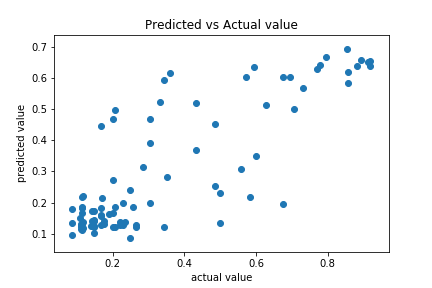
\includegraphics[width=0.75\linewidth]{./Images/ConvPredictedVAct.png}}
\caption{Predicted values generated by convolutional net vs actual value}
\label{fig:ConvPredictedVAct}
\end{figure}

Like with the single layer net, Fig. \ref{fig:ConvPredictedVAct} shows a linear correlation between the predicted values and human scores. However, as the human scores increase, we see a wider spread in predicted values when compared to the single layer net. 

\begin{figure}[htbp]
\centerline{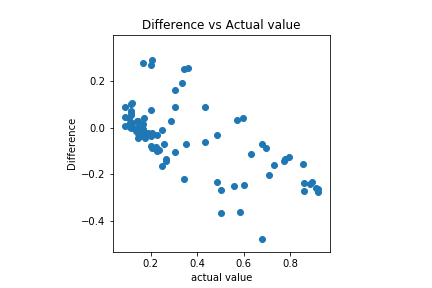
\includegraphics[width=0.75\linewidth]{./Images/ConvDiffVAct.png}}
\caption{Difference between predicted values generated by convolutional net and actual values vs actual value}
\label{fig:ConvDiffVAct}
\end{figure}

Once again, Fig. \ref{fig:ConvDiffVAct} shows that the convolutional net has a tendency to overscore worse models and underscore better models. However, when compared to the single layer net, we see a much tighter grouping of worse models (human scores $\leq0.3$) that the model was able to accurately guess with a difference of $-0.1 \leq$ Diff $\leq 0.1$. For the 90 image testing set, the convoltional net attained a mean difference of 0.112, which is slightly worse than the single layer net. 

\begin{figure}[htbp]
\centerline{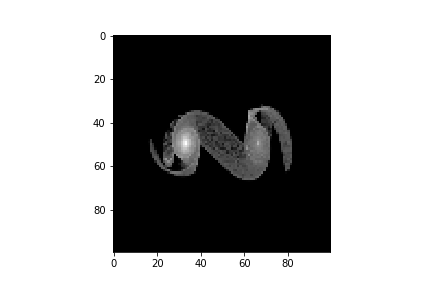
\includegraphics[width=0.75\linewidth]{./Images/ConvPredictedBest.png}}
\caption{Model that was scored the highest by the convolutional neural net}
\label{fig:ConvPredictedBest}
\end{figure}

Fig. \ref{fig:ConvPredictedBest} shows the image that was given the highest score by the convolutional net (0.695). This predicted value is significantly lower than the human score of 0.853, but it shows that the  convolutional net was still atleast somewhat successful in deciding on what the best model should look like. Once again, we can visually verify that the convolutional net's predicted best model closely resembles the target image shown in Fig. \ref{fig:TargetGalaxy}.

% DISCUSSION SECTION
\section{Discussion}

Both the single layer neural network and convolutional neural network show promise in correctly predicting how good of a fit a model is for a target galaxy collision. Both nets achieved a MSE of $\approx 0.02$ on the validation data and a mean difference of $\approx 0.1$ when tasked with predicting the scores of 90 test models. Both nets successfully chose an image out of a set of 90 that they decided was the best model for the target image. Upon visual comparison, these two chosen models very closely resemble the target galaxy collision. However, both models struggled with overfitting which can most likely be attributed to both our data set's small size and its uneven distribution of model quality. 

\begin{figure}[htbp]
\centerline{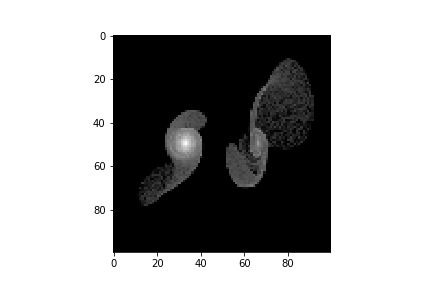
\includegraphics[width=0.75\linewidth]{./Images/ConvHumanNoiseExample.png}}
\caption{Example of a model that the convolutional net scored "poorly" when just comparing against human score.}
\label{fig:ConvHumanNoiseExample}
\end{figure}

Another factor to consider is the noise associated with the human scores. As a citizen scientist project, the models in the Galaxy Zoo: Mergers data set we ranked by people with minimal training. There are also no checks in place to prevent against people clicking though models without consideration, artificially inflating or deflating their scores. We must also acknowledge the randomness of the tournament system. It is entirely possible that some models were "unlucky" and went against rounds of exclusively good models, causing them to be scored lower than they actually should have or vice versa.

\begin{figure}[htbp]
\centerline{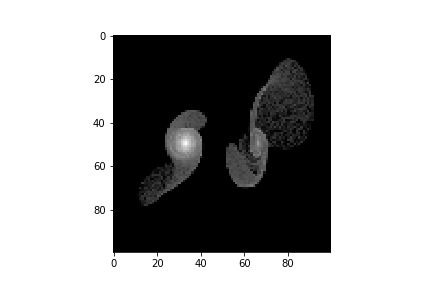
\includegraphics[width=0.75\linewidth]{./Images/ConvHumanNoiseExample.png}}
\caption{Example of a model that the convolutional net scored "poorly" when just comparing against human score.}
\label{fig:ConvHumanNoiseExample}
\end{figure}

Take for example the model shown in Fig. \ref{fig:ConvHumanNoiseExample}. This was one of the convolutional net's worst predictions, with a difference of nearly 0.5 between the net's predicted score of 0.195 and the human score of 0.676. However, if we visually compare this model with the target image, one could argue that the model did not deserve such a high human score. Instead, the model might better represent a score between the net's prediction and the human score. 

Future work could pertain to the expansion of the the convolutional nets to include more layers. Training with these extra layers and units would necessitate a larger data set, hopefully with a more even distributionn of model quality. We believe that such a net would obtain better results than either of the nets described in this paper.  Also, the nets we created for this paper could be applied to the other 61 galaxy pairs, and, with enough training, possibly eliminate the need for human rankings in the first place. This would allow for new models to be created and scored much faster than they have been previously. 


% REFERENCES
% THIS IS CREATED AUTOMATICALLY
\bibliographystyle{IEEEtran}
\bibliography{references} % change if another name is used for References file

\end{document}
